\begin{figure}[h]
\centering
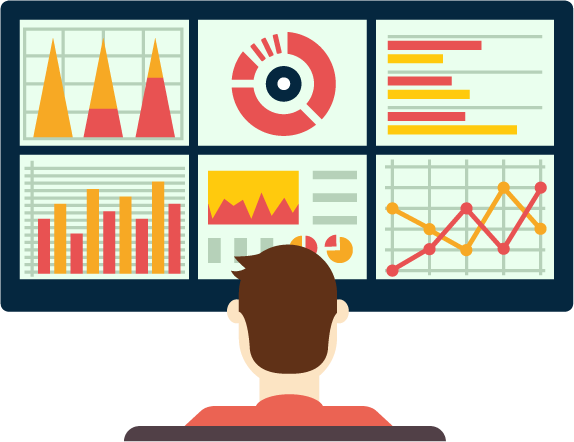
\includegraphics[scale=0.2]{figures/dashboard}
\end{figure}

\section{Monitoring CVMFS}
\paragraph{} This project can be used as a monitoring tool for cvmfs. send\_stats\_to\_graphite.py script should be called to send only the new stats data from the local database file to a tool that monitors and graphs numeric time-series data such as \href{https://graphiteapp.org/}{Grahite}.
\section{Alarm system}
\paragraph{} 
Different conditions can be verified in order to create an alarm system to discover unusual behaviour of the CVMFS. For example, a certain action could be started if no garbage collector process was registered. As an early success story for my project I can mention that on the 21st of August the garbage collector did not run (see figure 5.1), so I investigate the problem and I found out that the scripts that calls the garbage collector were updated that day.
\section{Benchmarking tool}
\paragraph{} By recording the start time and finished time of each publish or garbage collector action my project can help developers and the users of CVMFS to improve its performance. As we can see in the LHCb nightly test release manager statistics (see figure 5.5), the garbage collector run time is about two hours in average and it might be a good idea to reduce this in the future.  
